
\subsection{Introducción}

En esta sección se van a plasmar los diagramas de secuencia con una breve explicación de lo que está sucediendo con el fin de que narrando los hechos se comprenda de una manera más sencilla qué es lo que se está representando y facilitando en un futuro una reimplementación.

\subsection{Relativos a interacción con el Dispositivo}

\subsubsection{Flujo del Dispositivo}

En este diagrama se puede observar como fluye el dispositivo entre sus distintos estados.

La secuencia representada muestra como el dispositivo arranca directamente este servicio, el cual inicia sesión, o permanece intentándolo, para posteriormente enviar su estado.

Se muestra el flujo tando del caso de uso de \textit{inicio de sesión del dispositivo}, como del caso de uso de \textit{notificación de dispositivo conectado}, que están representados en los cuadros D01 y D02, respectivamente.

\begin{figure}[H]
    \centering
    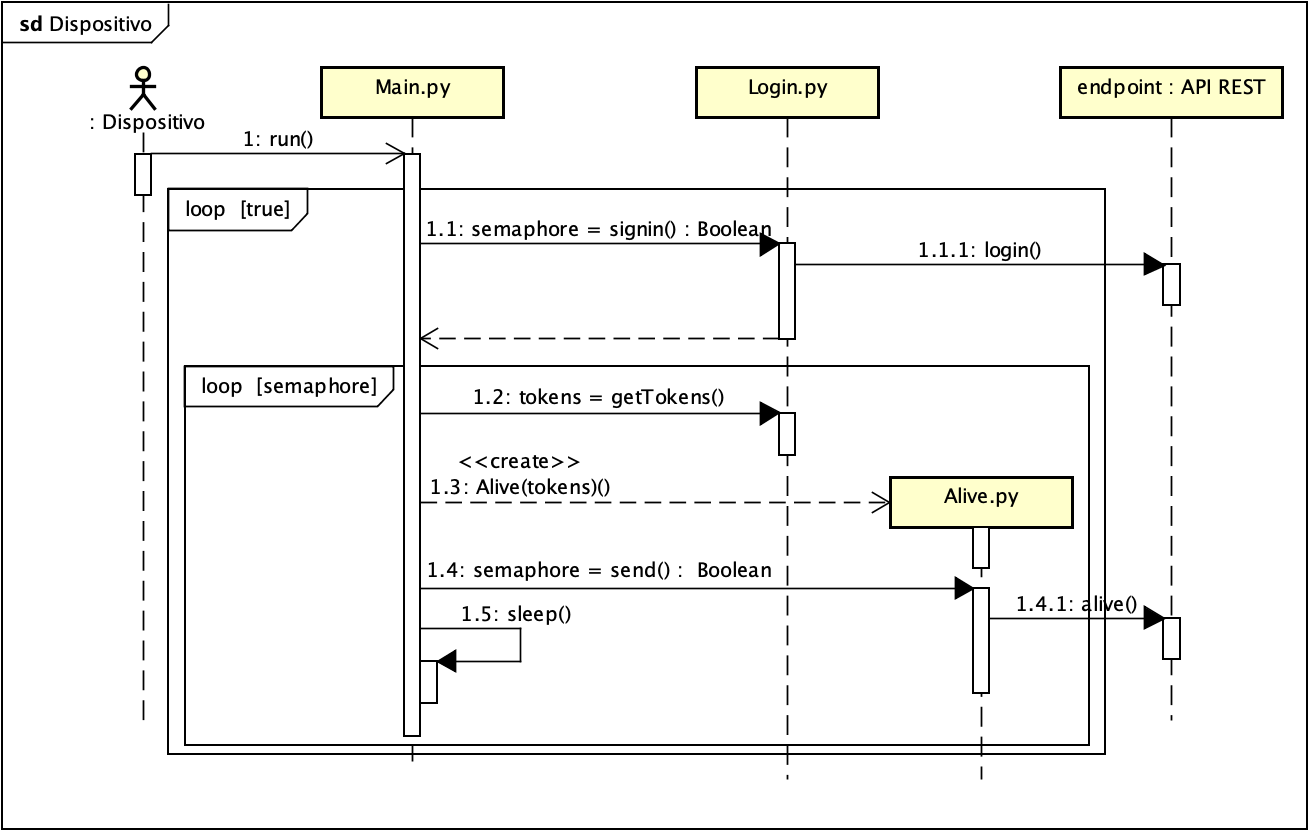
\includegraphics[width=12cm]{./img/sequence/diagram/device.png}
    \caption{Diagrama de secuencia DS01 - Dispositivo}
    \label{fig:seq.device}
\end{figure}

\subsubsection{Petición de Inicio de sesión}

En el siguiente diagrama de secuencia, el \textit{DS02}, se muestra la continuación del diagrama de secuencia anterior, haciendo incapié a qué es lo que ocurre en el lado del servidor una vez el dispositivo intenta iniciar sesión.

Como se puede observar, a un endpoint del servicio REST desplegado le llega una petición de inicio de sesión: un flujo correcto muestra cómo dentro del servidor, es el \textit{DeviceService} quien comprueba los credenciales, que siendo correctos sigue el flujo de secuencia y se solicita unos nuevos tokens para un dispositivo concreto al servicio de autenticación.

Si observamos la capa de dominio del servidor, que llamaremos \textit{core}, está basada en la implementación de unas interfaces que están definidas en el propio core. De esta forma cualquer servicio que en un futuro se quiera usar deberá implementar estas interfaces. Así se asegura la integridad del sistema, permitiendo cambiar de servicio en un futuro sin necesidad de tocar el core, manteniendo la misma funcionabilidad del sistema.

\begin{figure}[H]
    \centering
    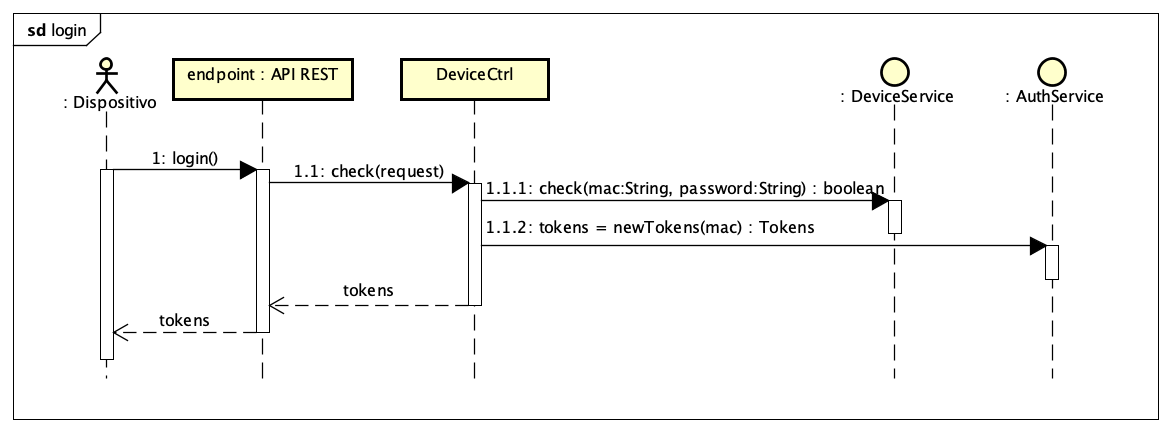
\includegraphics[width=14cm]{./img/sequence/diagram/login.png}
    \caption{Diagrama de secuencia DS02 - Login}
    \label{fig:seq.login}
\end{figure}

\subsubsection{Petición de Dipositivo conectado}

El diagrama de secuencia \textit{DS03}, representado en la figura \ref{fig:seq.alive}, muestra también el comportamiento del servidor tras otra petición.

En este caso se trata de una petición de aviso de que el dispositivo está conectado, documentada en el cuadro \textit{D02}, la cual se puede observar que tiene finalmente dos posibles finales correctos: la finalización, y la realización del caso de uso de \textit{realización de tarea pendiente}, el cual está plasmado en el caso de uso \textit{D03}.

En este diagrama se expone cómo el dispositivo realiza la petición, y tras esa petición, el servidor se encaga de comprobar primero si el token del dispositivo es correcto para posteriormente decirle al controlador de tareas, \textit{TaskCtrl}, que el dispositivo acaba de realizar la tarea de mostrar que está conectado.

El controlador de tareas almacena el nuevo estado del dispositivo para posteriormente recuperar todas las tareas pendientes, que en caso de no haber alguna, se responde al dipositivo con un código de estado HTTP cuyo valor es 200, finalizando el caso de uso.
En cambio, si el controlador sí que ha recibido tareas pendientes, se le responde al dispositivo un código 300, disparando un nuevo caso de uso en el dispositivo, el cual es la realización de tareas pendientes, como se ha nombrado anteriormente.

\begin{figure}[H]
    \centering
    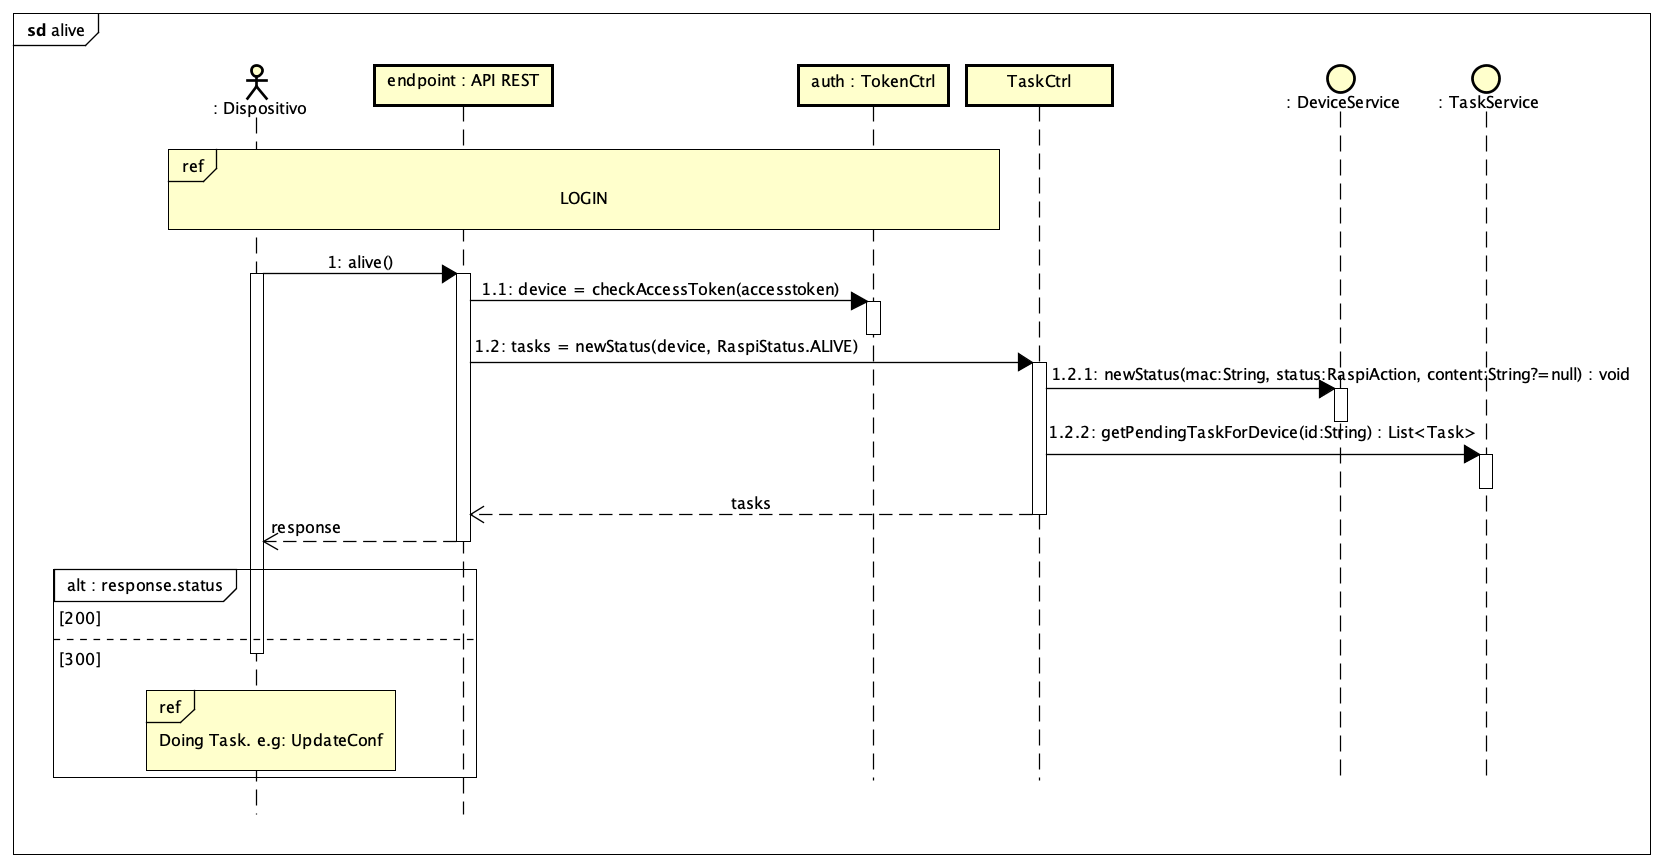
\includegraphics[width=14cm]{./img/sequence/diagram/alive.png}
    \caption{Diagrama de secuencia DS03 - Alive}
    \label{fig:seq.alive}
\end{figure}

\subsubsection{Realización de Tareas pendientes}

El presente diagrama de secuencia muestra el un prototipo de flujo válido a implementar en los dispositivos para implementación del caso de uso de \textit{Realización de tarea pendiente D03}, siendo válido para cualquier tipo de tarea, que en este caso representará a la tarea configuración, la cual está asociada también al caso de uso de \textit{actualización de la configuración D04}, ya que esta tarea es un requisito indispensable del sistema, y de este modo se puede mostrar mejor la combinación de ambas dando como resultado la posibilidad de actualizar y controlar remotamente el dispositivo.

En esta representación gráfica de la secuencia por la cual se realiza el caso de uso, se observa que previamente el dispositivo ha recibido una respuesta del servidor a una \textit{petición de dispositivo conectado} la cual contiene un código de estado de código 300, la cual se comprueba y se obtiene del cuerpo del mensaje las tareas pendientes.

Una vez se tienen las tareas, se forma un comando, como se narra en el apartado \ref{seq:received300}, y es ejecutado contra el sistema.

Este comando hace que el sistema ejecute un script, \textit{init.sh}, el cual arranca la realización de la tarea, en este caso la de actualizar la configuración, la cual está implementada en \textit{Conf.py}.

La tarea primero avisa al servidor que procede a realizar la tarea pendiente, que si recibe un mensaje correcto \textit{-código 200-} procede a realizar la tarea solicitada.

Por tanto, la tarea de configuración solicitará al servidor el archivo de configuración, que en caso de recibirlo, actualizará el fichero.

Una vez actualizado, si todo ha sido correcto, avisa al servidor sobre su finalización, de manera que el servidor marcará la tarea como realizada.

En esta secuencia se puede observar un protocolo de actuación a la hora de tratar las tareas:

\begin{enumerate}
    \item Avisar que se va a hacer la tarea.
    \item Hacer la tarea.
    \item Avisar que se ha hecho la tarea.
\end{enumerate}

Gracias a este protocolo un administrador puede observar si una tarea no ha sido realizada porque no le ha llegado, o porque no ha sido capaz de realizarla, dando la posibilidad a una mejor gestión de los problemas.

\begin{figure}[H]
    \centering
    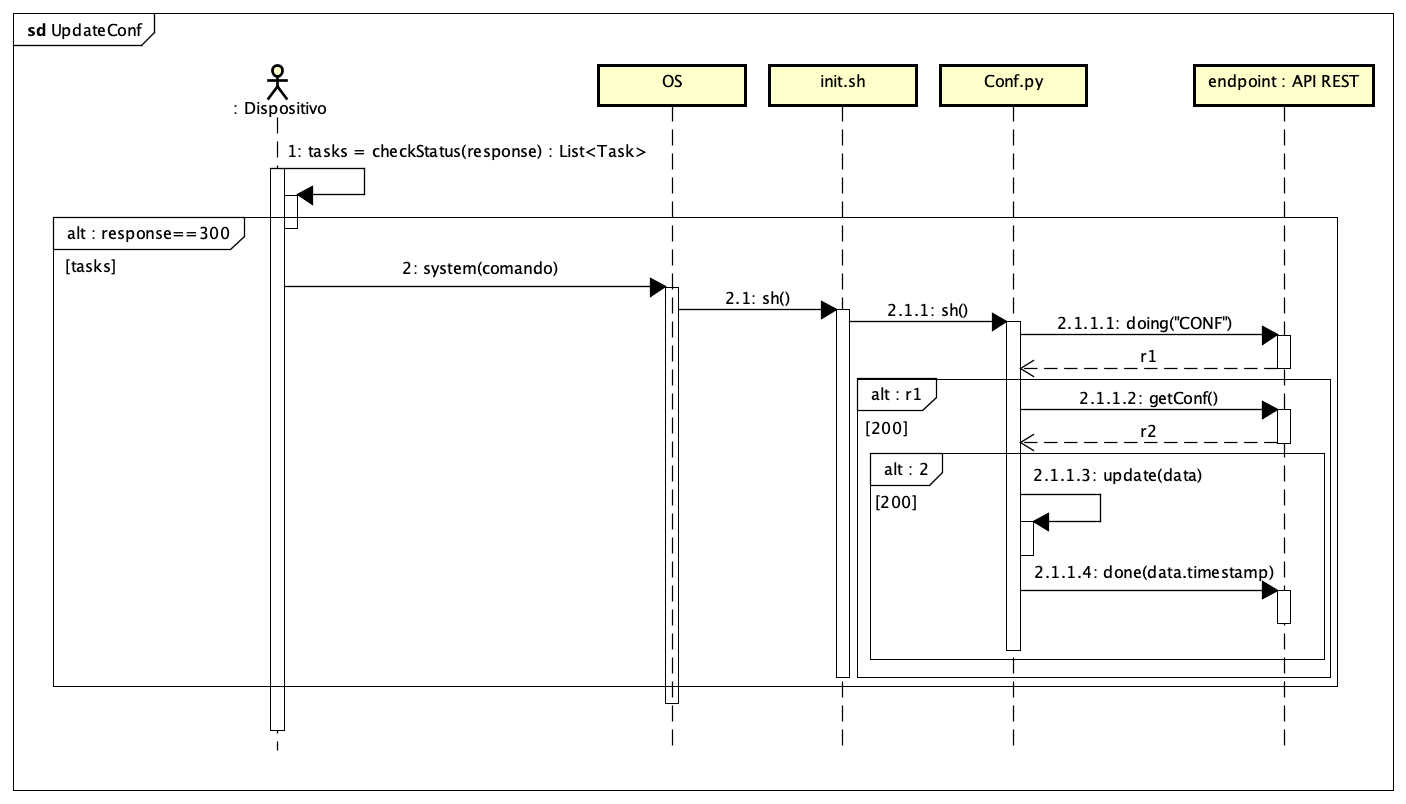
\includegraphics[width=14cm]{./img/sequence/diagram/conftask.png}
    \caption{Diagrama de secuencia DS04 - Realización de tareas pendientes}
    \label{fig:seq.alive}
\end{figure}

\subsubsection{Marcar Tarea como Realizada}

Tras comprobar en el servidor la validez del token con el cual se hace la petición y obtener el dispositivo asociado, se almacena un nuevo estado del dispositivo, para su visualización de a qué hora se ha realizado la acción y poder observar su actividad. Posteriormente se marca esa tarea como finalizada, asignándole la hora en la cual se ha recibido en el servidor.

\begin{figure}[H]
    \centering
    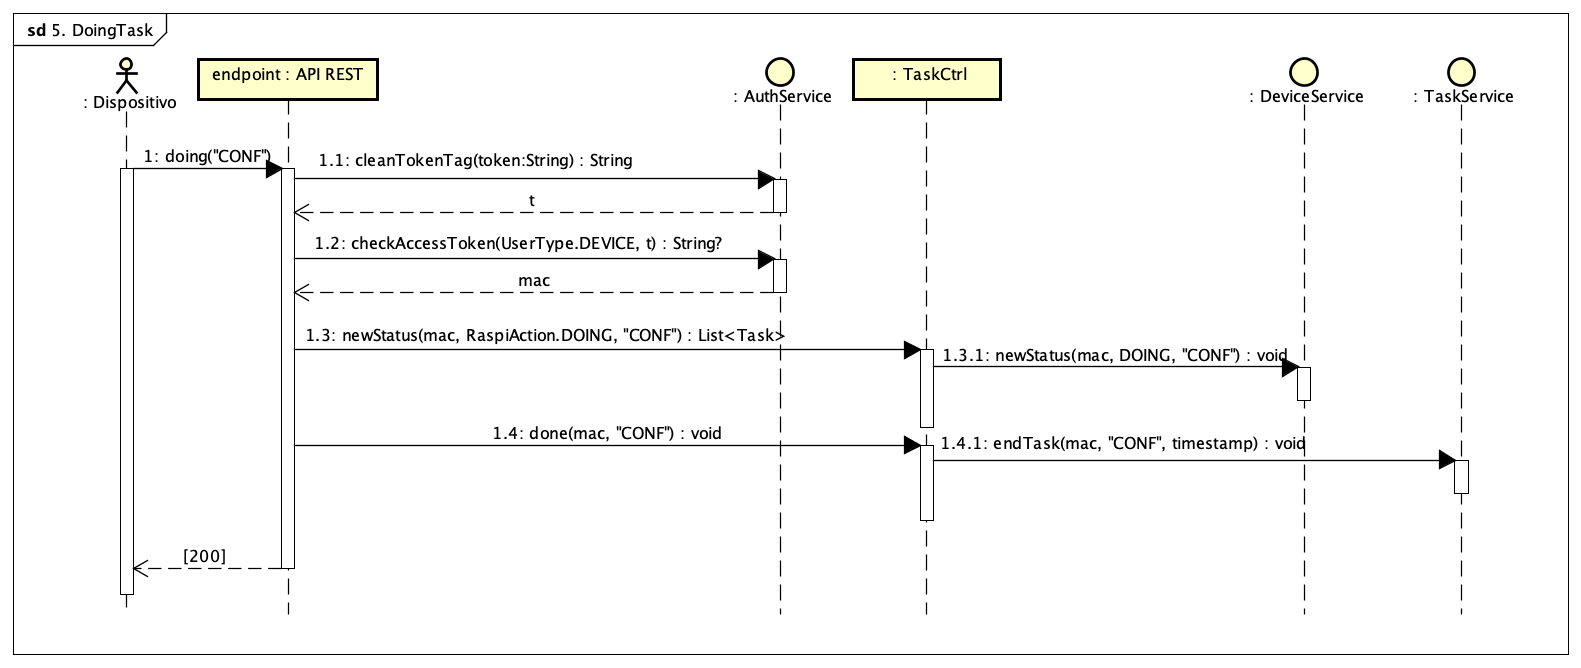
\includegraphics[width=14cm]{./img/sequence/diagram/doingTask.png}
    \caption{Diagrama de secuencia DS05 - Servidor : Marcar tarea como realizada}
    \label{fig:seq.doing}
\end{figure}


\subsubsection{Marcar la Configuración de un dispositivo como Actualizada}

La siguiente secuencia representa una de las acciones con mayor complejidad del sistema, ya que poder llevar el registro de cual es la configuración que posee cada dispositivo y a cual es a la que se ha actualizado, teniendo en cuenta que hay 3 posibles configuraciones paralelas, lleva un tedioso trabajo, que una vez clarificado no es difícil de entender.

Partimos de que el dispositivo informa que ha actualizado a la configuración que posee una marca de tiempo específica.

Entonces, el sistema obtiene las configuraciones globales, locales y propias que corresponden a cada dispositivo y comprueba:

Si el timestamp corresponde con la global, elimina todas las configuraciones globales, ya estén pendientes o no, asignadas a ese dispositivo, y añade la actualizada como no pendiente.

Si no corresponde con la global, si no que con la local, elimina todas las configuraciones locales asignadas a ese dispositivo, estén pendientes o no, y añade la actualizada como no pendiente.

Si tampoco corresponde con la local, si no que corresponde con la propia del dispositivo, elimina la configuración no pendiente asignada, y cambia el estado de la pendiente.

\begin{figure}[H]
    \centering
    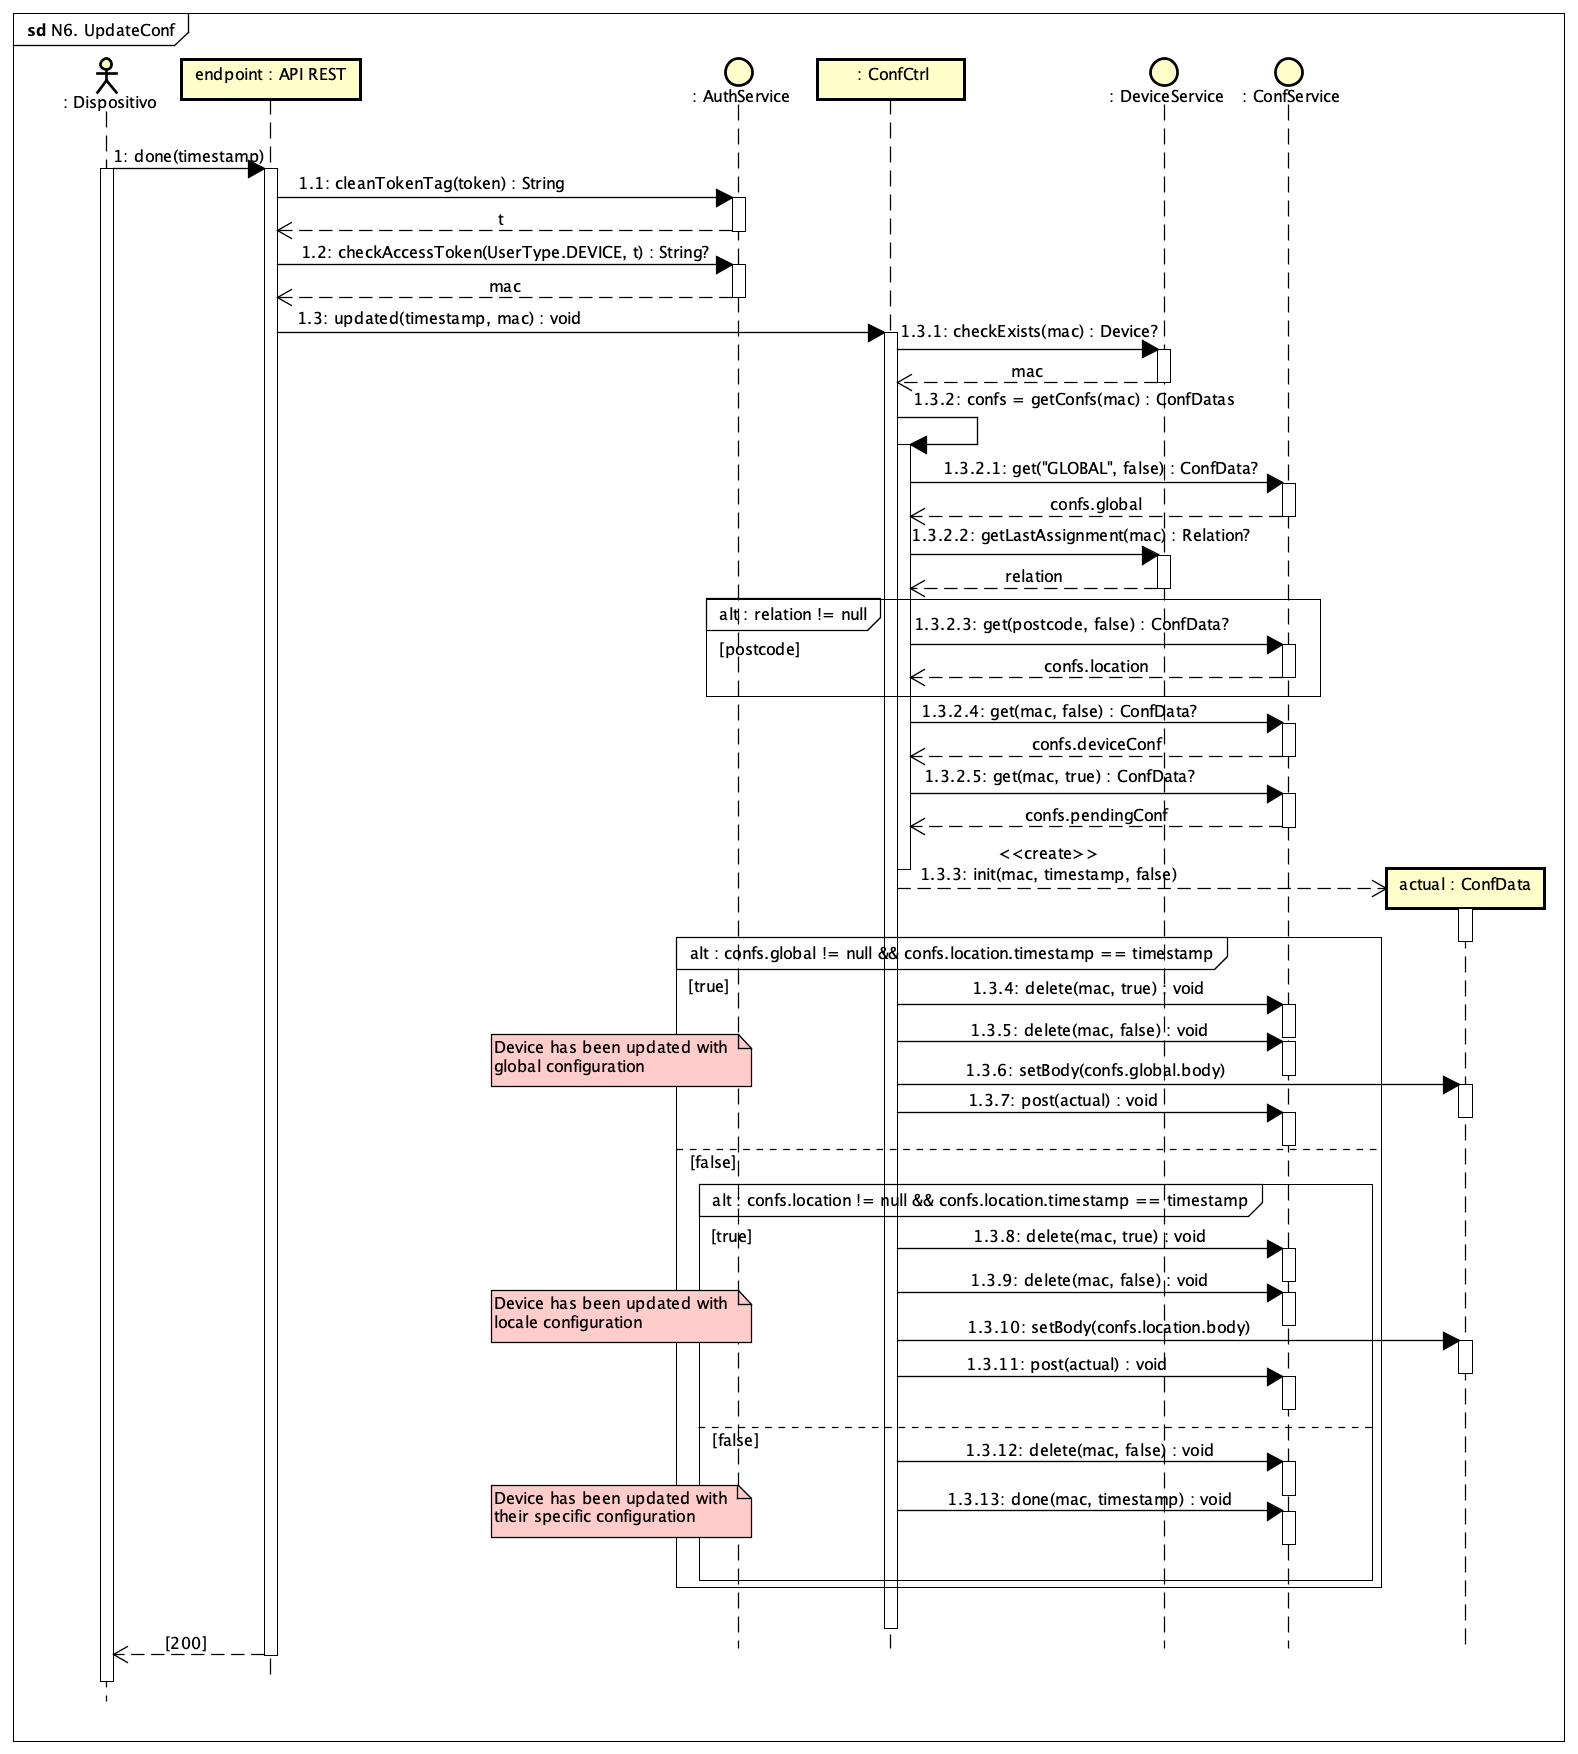
\includegraphics[width=14cm]{./img/sequence/diagram/updateConf.png}
    \caption{Diagrama de secuencia DS06 - Servidor : Configuración actualizada}
    \label{fig:seq.UpdateConf}
\end{figure}

\newpage
\subsubsection{Obtención de la Configuración Actual}

Para obtener la configuración de un dispositivo, el sistema simplemente obtiene el identificador correspondiente al token de la cabecera, del cual recolecta los datos, como si tiene ese dispositivo un usuario asociado.

A partir de esos datos, recoge la configuración global, la local a partir de la asignación de usuario si posee, y la del propio dispositivo, tanto la pendiente como la instalada. De todas estas configuraciones se queda con la que tenga el timestamp más actual, de modo que será la que debe ser enviada.

Si la marca de tiempo de la que se va a devolver es más reciente que la que está guardada como la actual del dispositivo, se marca la que se devuelve como que tiene pendiente su instalación.
\newpage

\begin{figure}[H]
    \centering
    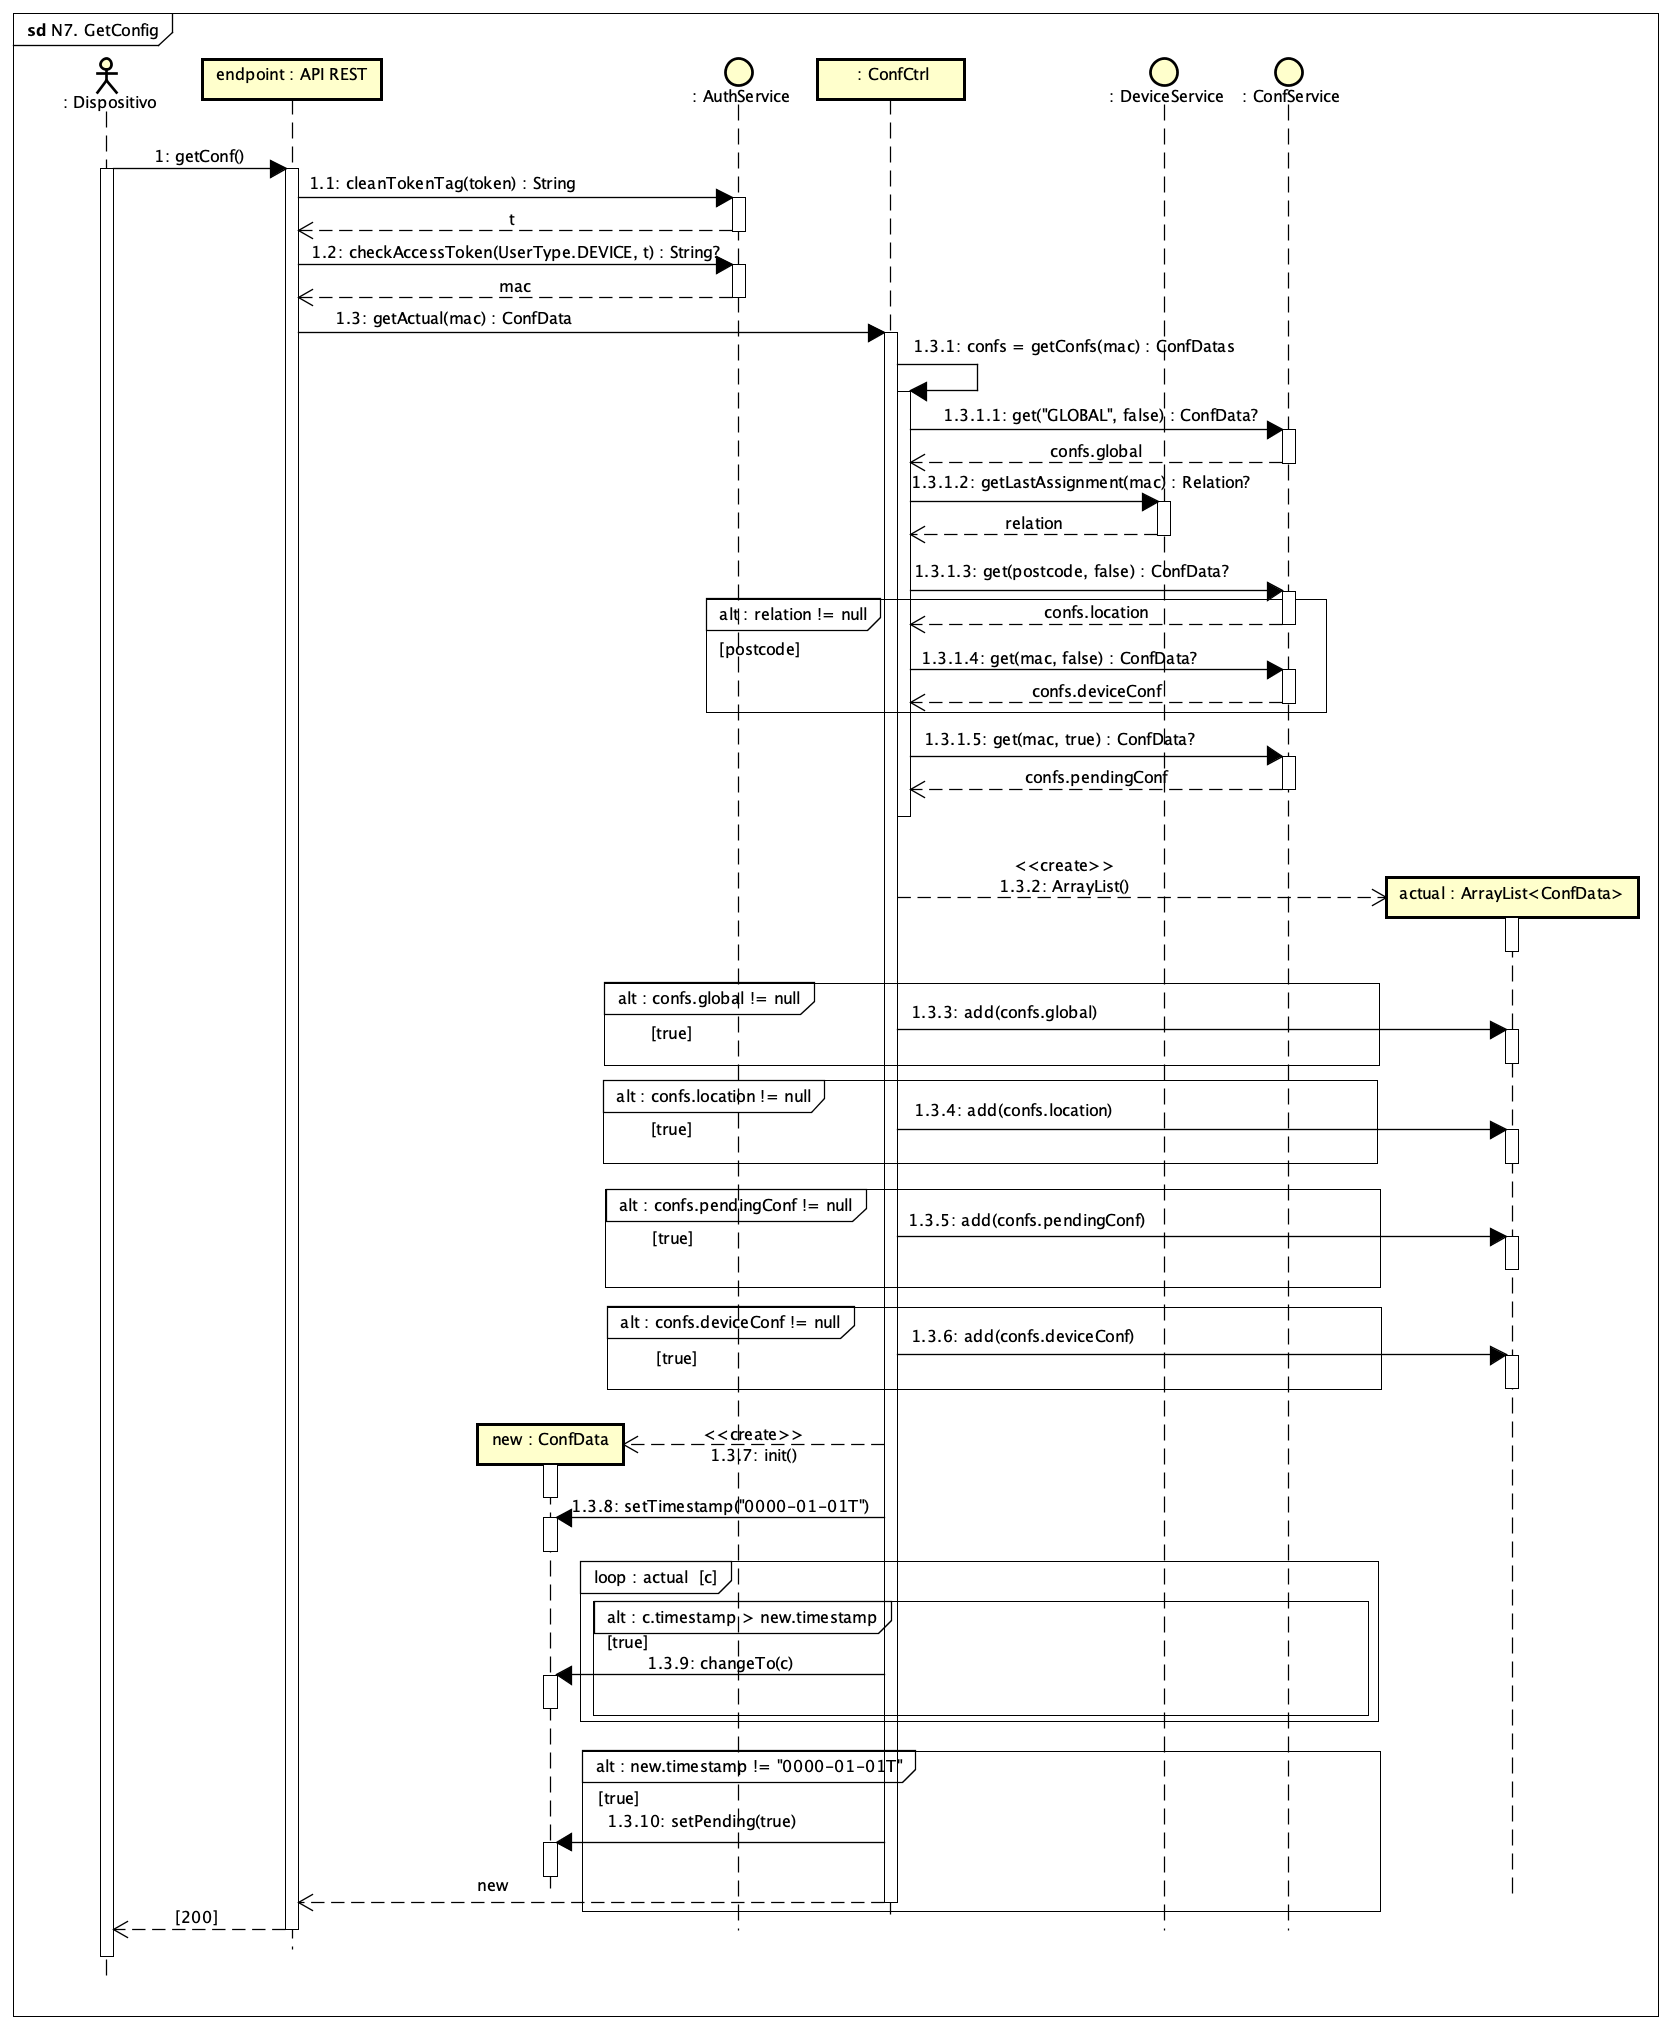
\includegraphics[width=14cm]{./img/sequence/diagram/getConfig.png}
    \caption{Diagrama de secuencia DS07 - Servidor : Obtener configuración actual}
    \label{fig:seq.GetCurrentConf}
\end{figure}

\subsection{Relativos a la Interacción de un Administrador}

\subsubsection{Creación de un nuevo Tipo de Tarea}

La creación de nuevas tareas en el dispositivo ha sido explicado previamente en el apartado \ref{seq:received300}, pero para poder mandar al dispositivo esa nueva tarea, hay que poder registrarla en el sistema.

En la siguiente secuencia se muestran los pasos por los cuales un nuevo tipo de tarea puede ser registrada, permitiendo posteriormente la asignación a los dispositivos.

En este caso, para diferenciar entre la creación de tipos de tareas y la creación de una asignación de tarea a los dispositivos, modificaremos el nombre de referencia, llamando a los tipos de tareas  \textit{eventos}, y a la asignación de dichos eventos a los dispositivos, \textit{tareas}.

\begin{figure}[H]
    \centering
    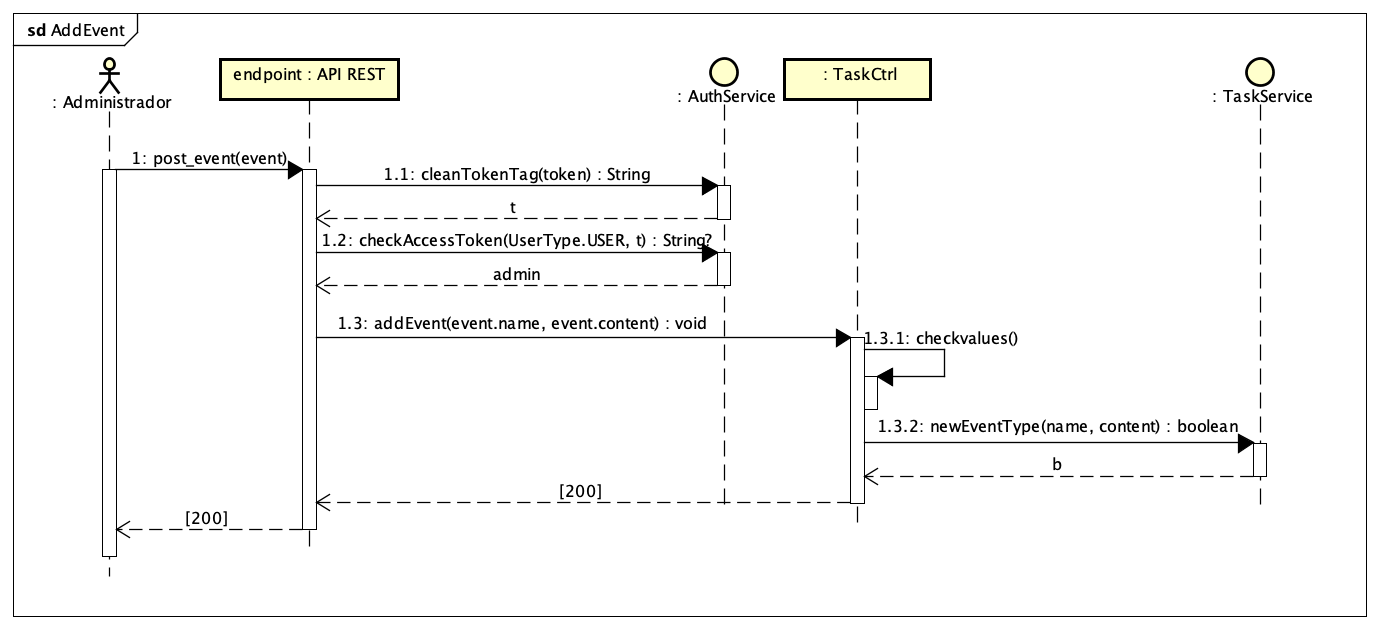
\includegraphics[width=14cm]{./img/sequence/diagram/AddEvent.png}
    \caption{Diagrama de secuencia DS08 - Creación de nuevo tipo de tarea}
    \label{fig:seq.NewEvent}
\end{figure}

\newpage
\subsubsection{Asignación de una Tarea a un Dispositivo}

Una vez se ha mostrado cómo puede ser la estructura del dispositivo para realizar las tareas, y se ha dado la posibilidad de crear eventos en el servidor, solo falta mostrar como son asignables esos eventos a los dispositivos generando nuevas tareas.

\begin{figure}[H]
    \centering
    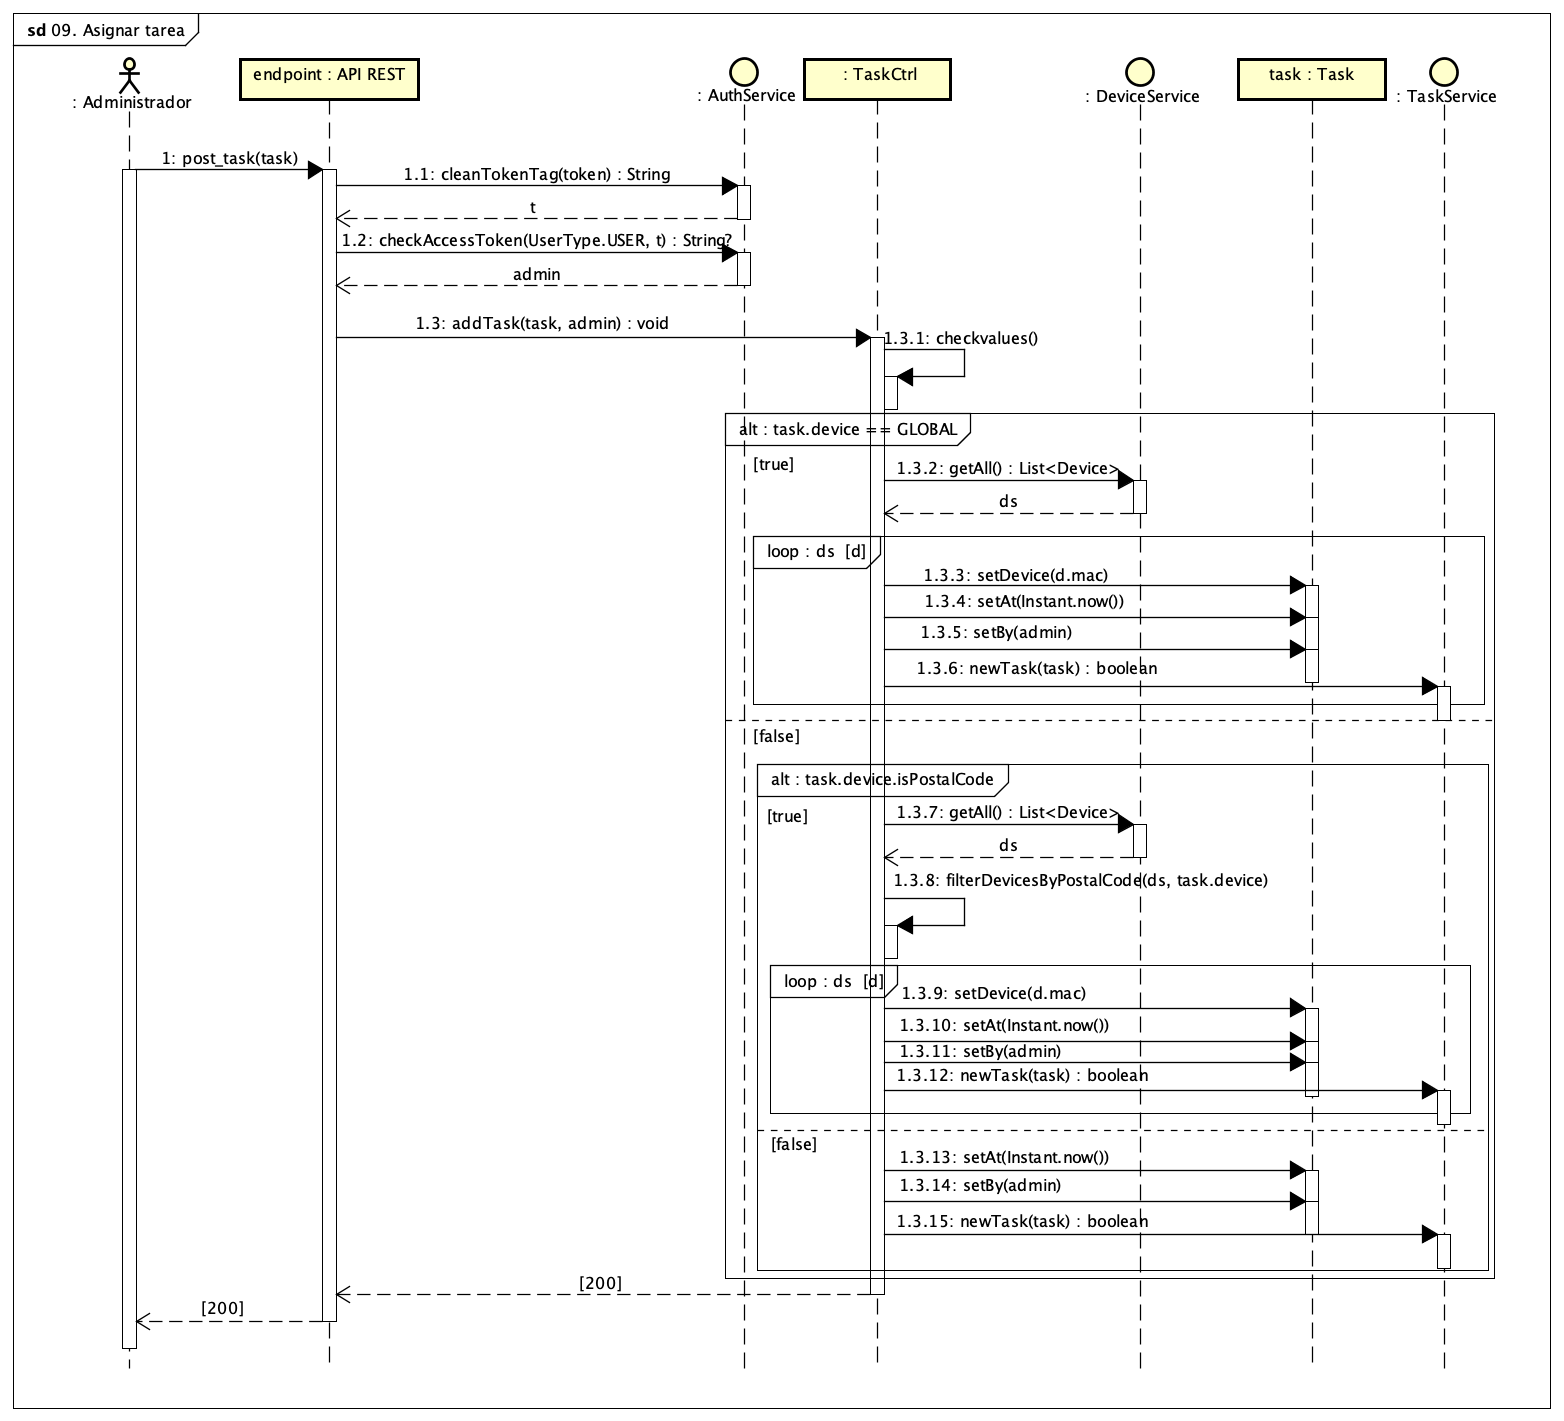
\includegraphics[width=14cm]{./img/sequence/diagram/AssignTask.png}
    \caption{Diagrama de secuencia DS09 - Asignación de tarea a dispositivo}
    \label{fig:seq.AssignTask}
\end{figure}

\newpage
\subsubsection{Recolección de Eventos}
Como bien se ha definido en los requisitos y se ha estipulado en el caso de uso \textit{A04}, un administrador debe poder obtener la lista completa de eventos del sistema, con el fin de saber cuáles están ya definidos y pueden ser asignados a los dispositivos.

\begin{figure}[H]
    \centering
    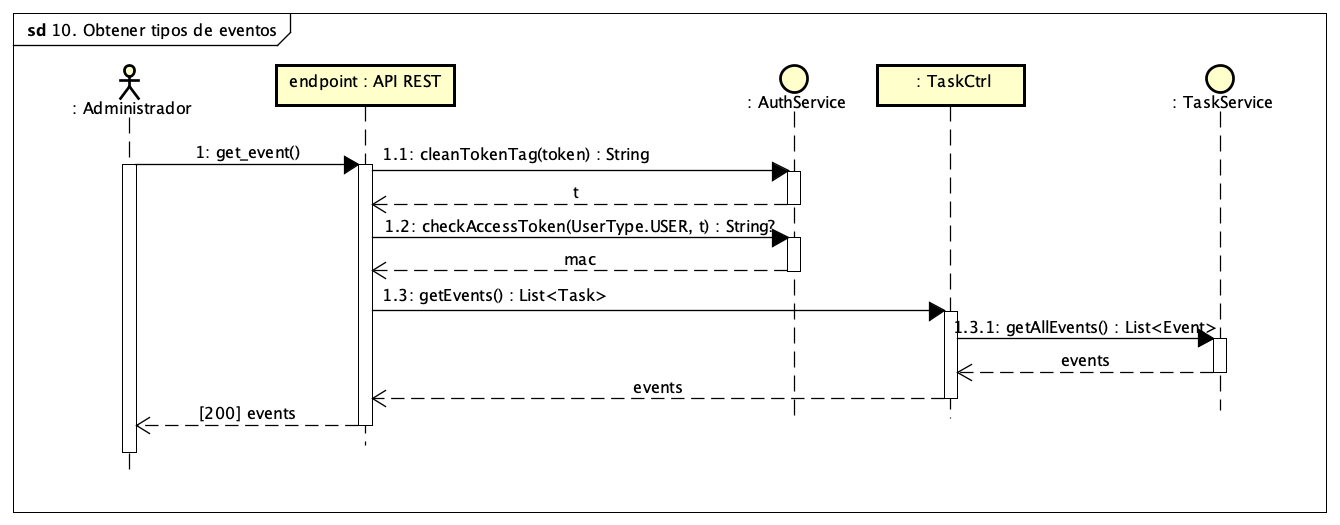
\includegraphics[width=14cm]{./img/sequence/diagram/GetEvents.png}
    \caption{Diagrama de secuencia DS10 - Recolección de eventos}
    \label{fig:seq.GetEvents}
\end{figure}

\subsubsection{Obtención de Tareas de un Dispositivo}

En los requisitos funcionales se data la necesidad de un método que permita la obtención de todas las tareas que han sido asignadas a un dispositivo en un determinado rango de tiempo, por lo que en el siguiente diagrama de secuencia se muestra la implementación.

\begin{figure}[H]
    \centering
    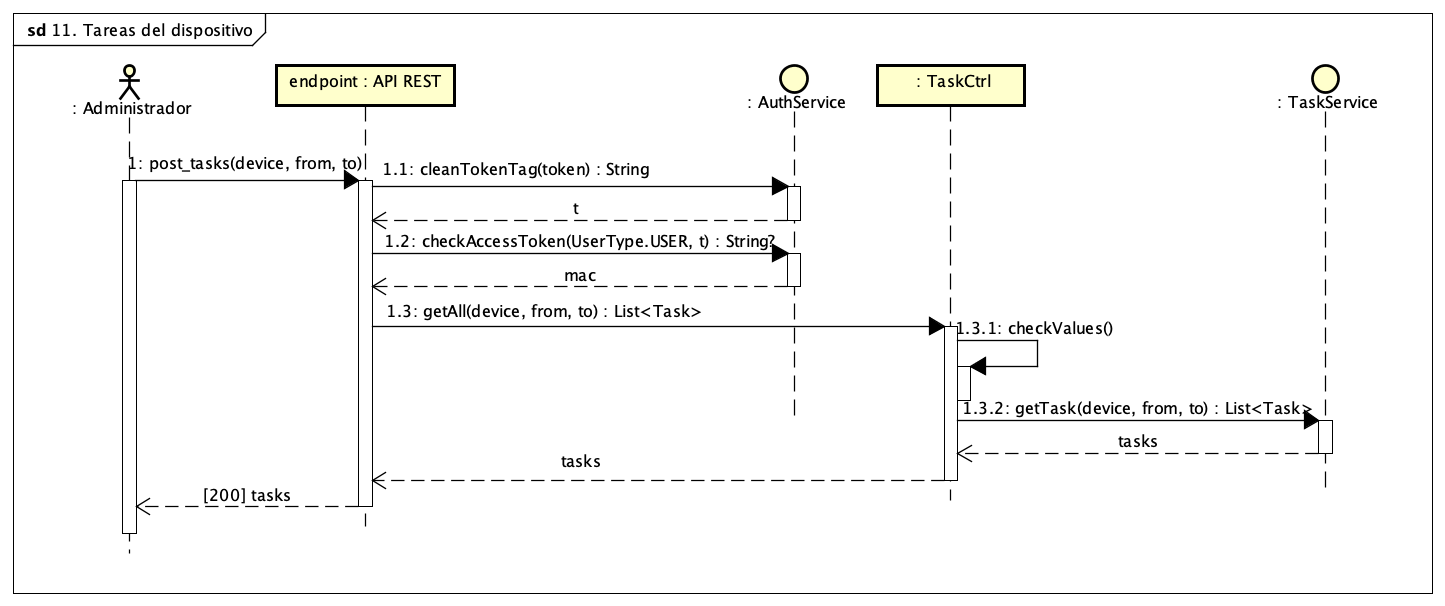
\includegraphics[width=14cm]{./img/sequence/diagram/TareasDeDispositivo.png}
    \caption{Diagrama de secuencia DS11 - Obtención de tareas de un dispositivo}
    \label{fig:seq.getDeviceTasks}
\end{figure}

\newpage
\subsubsection{Cambiar Configuración}

El administrador es capaz de cambiar la configuración tanto global, como local o de un dispositivo específico a través de una llamada a un endpoint del servicio REST del sistema.
Lo que ocurre en el sistema una vez se realiza la petición es documentado en el siguiente diagrama de secuencia.

\begin{figure}[H]
    \centering
    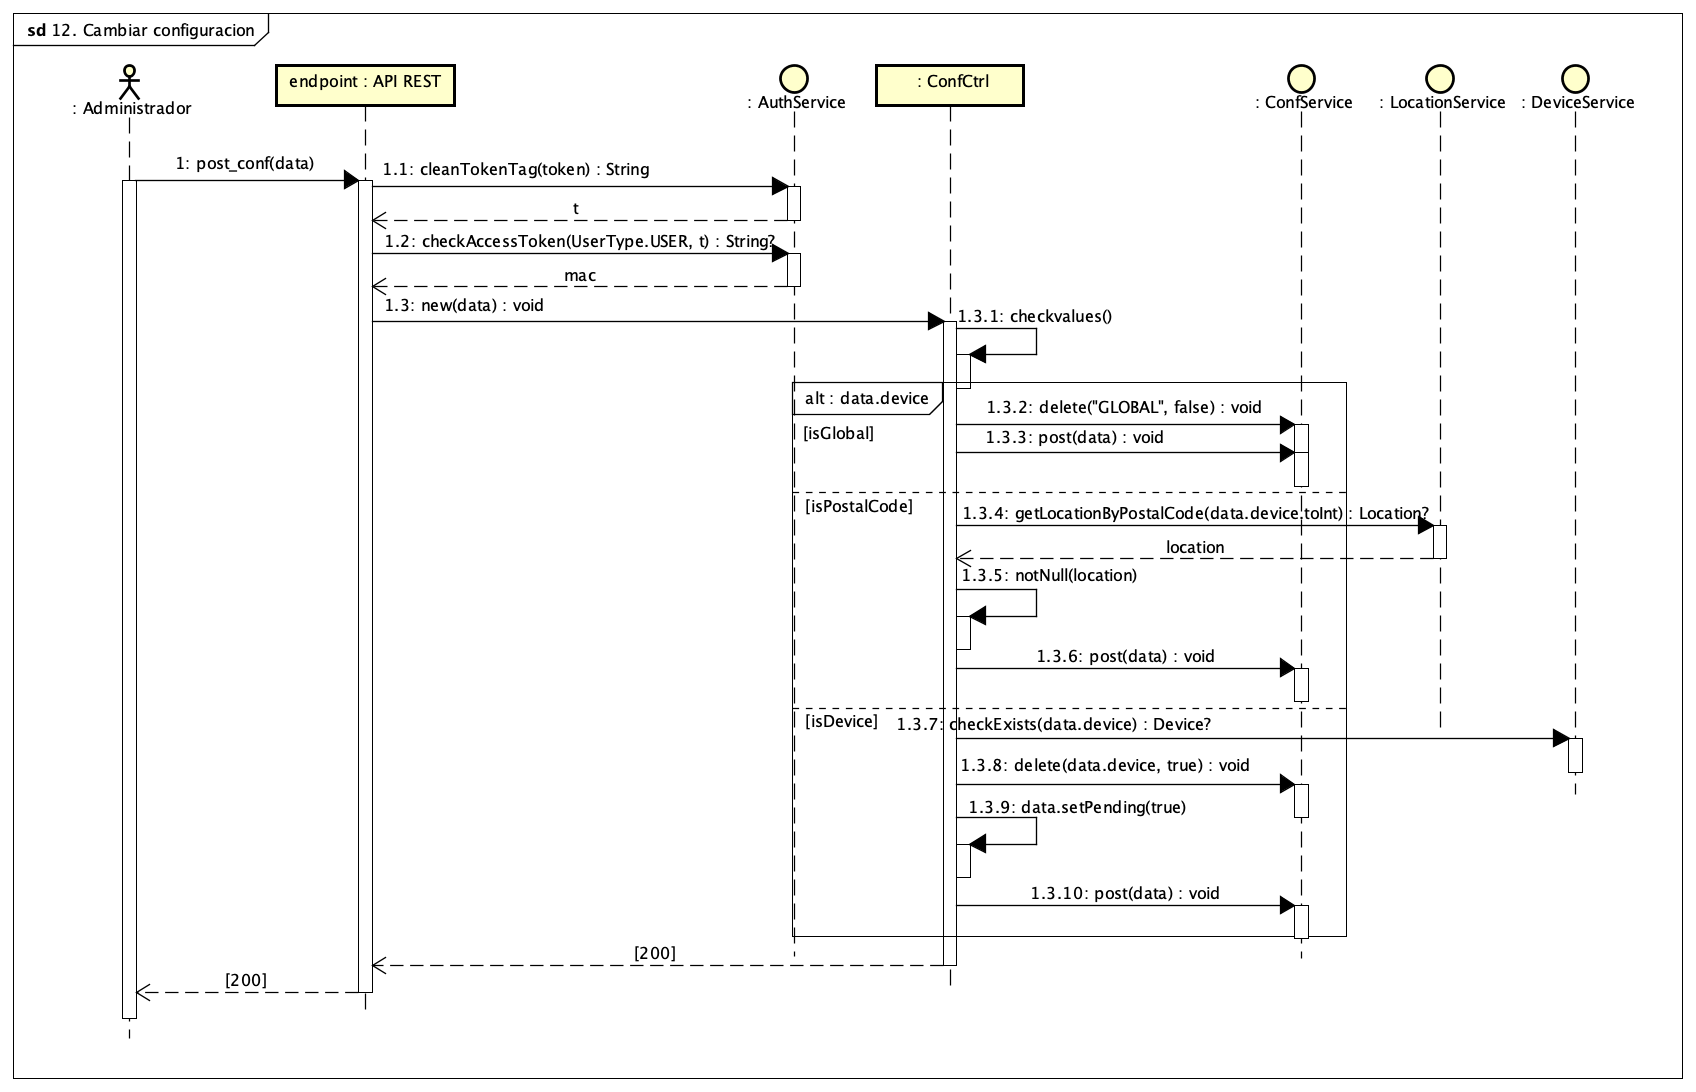
\includegraphics[width=14cm]{./img/sequence/diagram/CambiarConfiguracion.png}
    \caption{Diagrama de secuencia DS12 - Cambiar configuración}
    \label{fig:seq.ChangeConf}
\end{figure}

\newpage
\subsubsection{Obtención de todos los Dispositivos}

Para poder llevar un registro del estado actual de los dispositivos y ver si alguno está dando algún tipo problema es necesario poder obtener todos los dispositivos.
El siguiente diagrama de secuencia muestra cómo el sistema recoge primero todos los dispositivos que contiene, para posteriormente añadir a cada uno de ellos información como cuáles han sido los últimos estados que ha enviado, o cuáles son las últimas 5 tareas que ha realizado. También, cuáles han sido los últimos \textit{intents} que ha realizado, representando un intent a la interación entre usuario y dispositivo, al igual que obtiene las tareas pendientes que tiene cada dispositivo.

\begin{figure}[H]
    \centering
    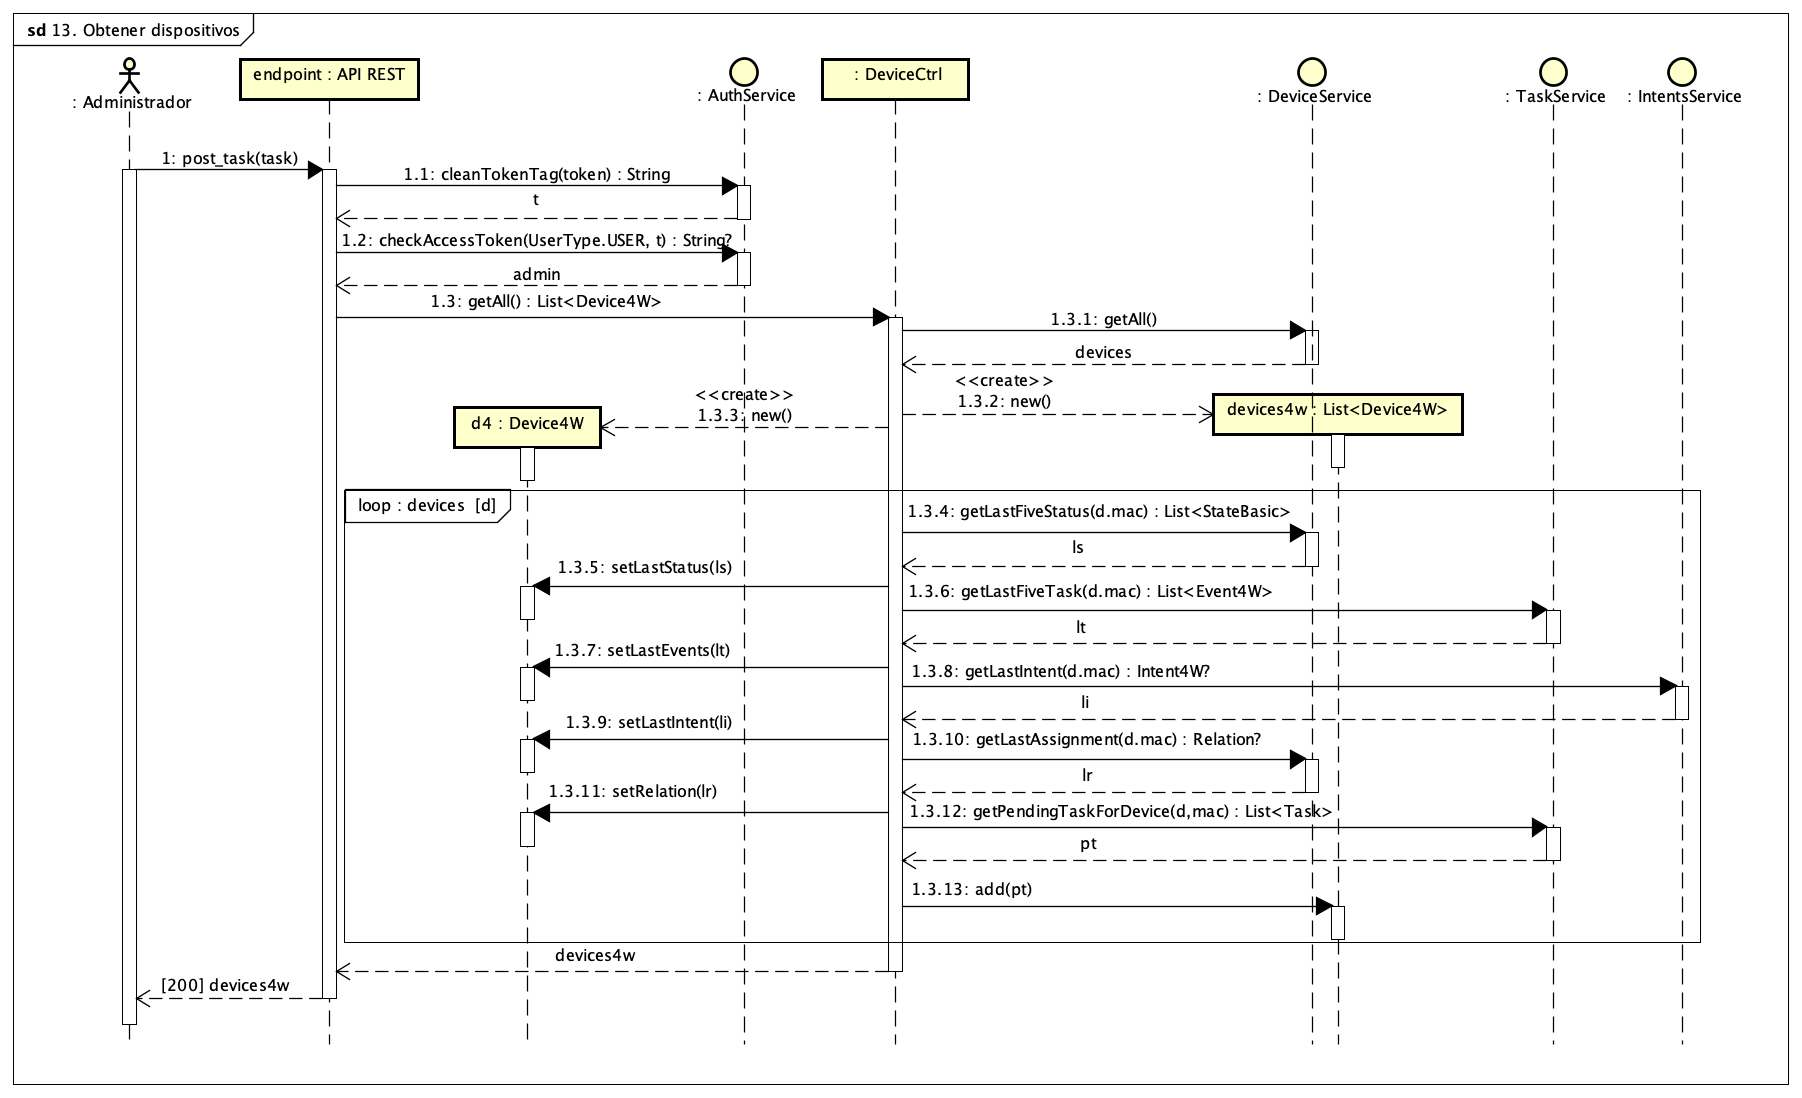
\includegraphics[width=14cm]{./img/sequence/diagram/ObtenerDispositivos.png}
    \caption{Diagrama de secuencia DS13 - Obtención de todos los dispositivos}
    \label{fig:seq.GetDevices}
\end{figure}

\newpage
\subsubsection{Obtención de Actividad}

Un requisito del sistema era la necesidad de un servicio que obtuviese la actividad relacionada con un dispositivo en un periodo establecido, pero también la implementación de un servicio que obtuviese la actividad de un determinado usuario.

Por motivos de seguridad, se ha implementado la obtención de la actividad de un dispositivo, de la cual se puede obtener la sucedida entre cualquier periodo de fechas siempre y cuando no tenga ningún usuario asociado.

En caso de que un dispositivo tenga un usuario asociado en el momento de la consulta, los resultados se limitarán a mostrar la actividad de ese dispositivo únicamente con el usuario actual.

De este modo, como se puede observar en el diagrama de secuencia incluido a continuación, se evita la posibilidad de que un usuario acceda a consultas de actividades hechas con el mismo dispositivo por otro usuario, al igual que no permite obtener a los administradores la actividad de un determinado usuario, si el usuario ya no tiene el dispositivo asignado, respetando por tanto la privacidad.

\begin{figure}[H]
    \centering
    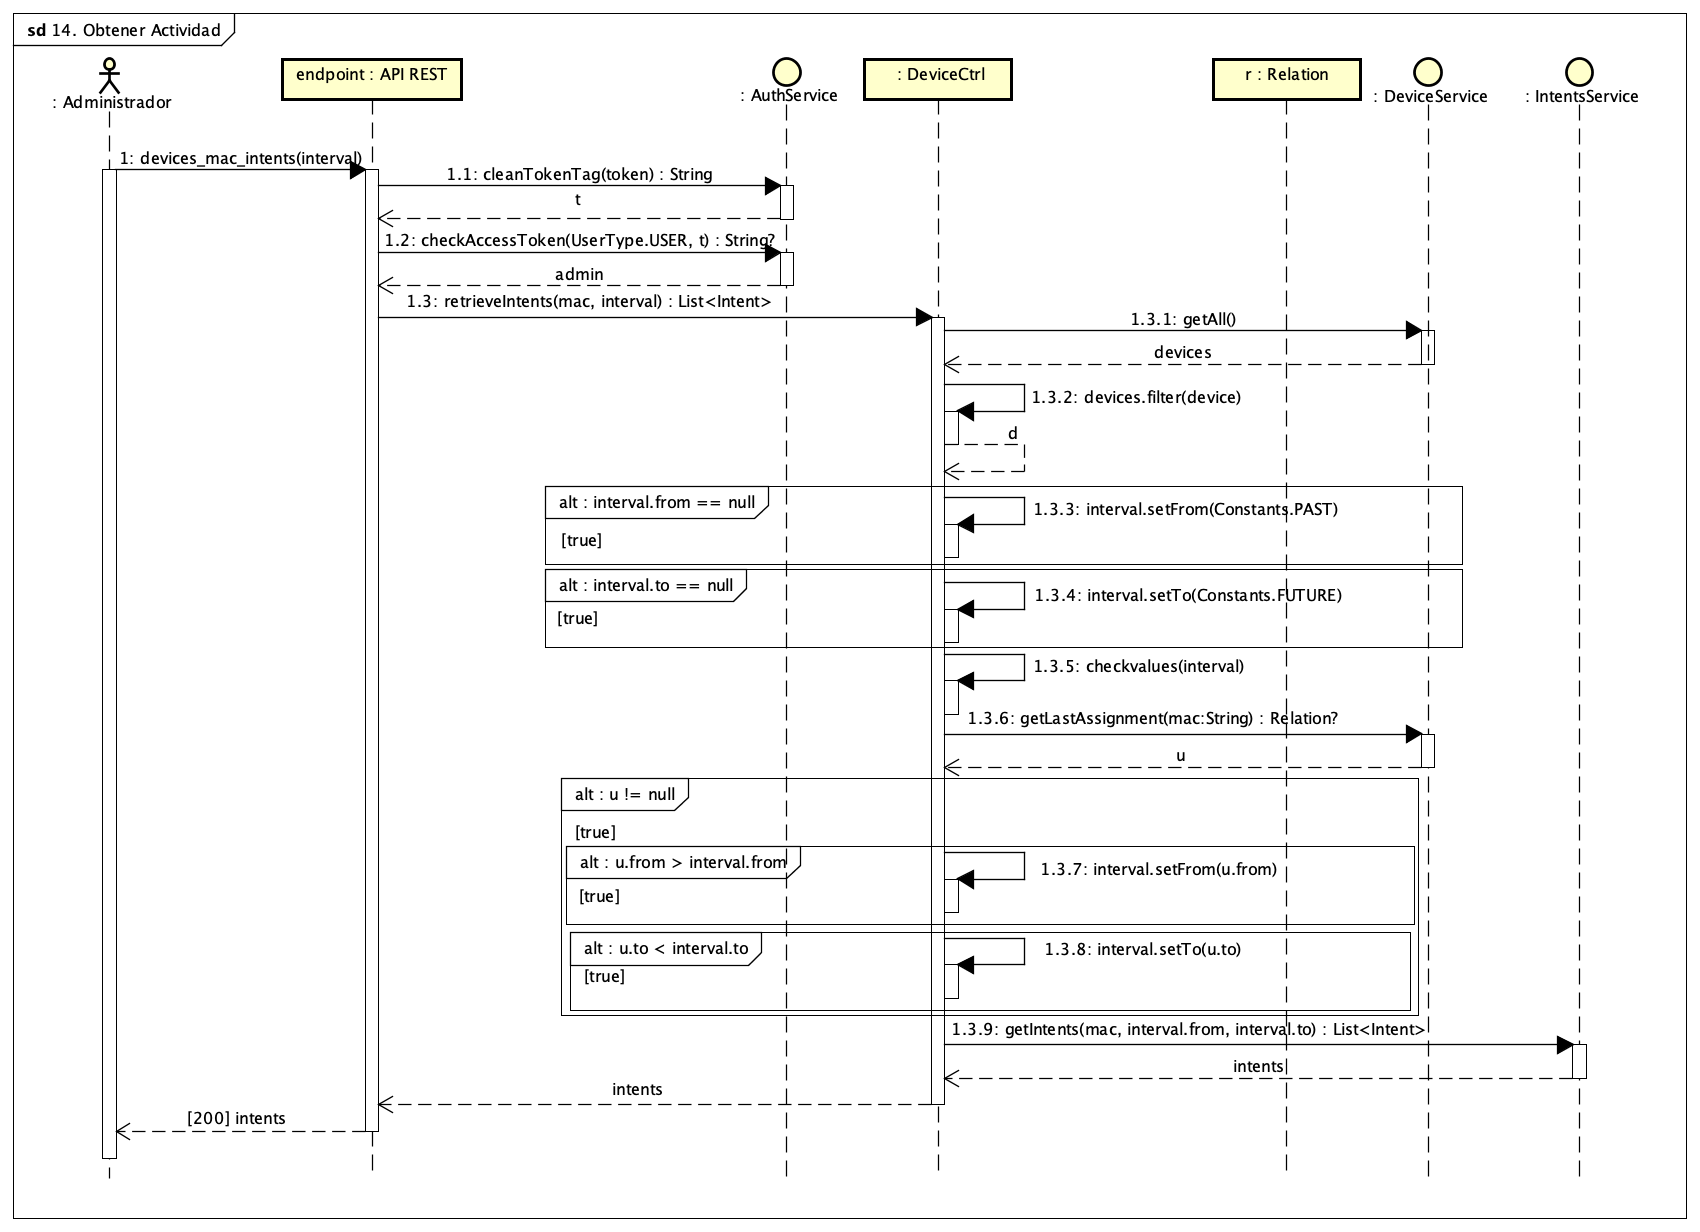
\includegraphics[width=14cm]{./img/sequence/diagram/ObtenerActividad.png}
    \caption{Diagrama de secuencia DS14 - Obtención de actividad}
    \label{fig:seq.GetTask}
\end{figure}


\subsubsection{Adición de una Nueva Localidad}

Con el fin de una mejor organización del sistema, se debe poder añadir la localidad en la cual se esté operando. De este modo, los dispositivos y usuarios pueden estar asociados a una localidad específica.

\begin{figure}[H]
    \centering
    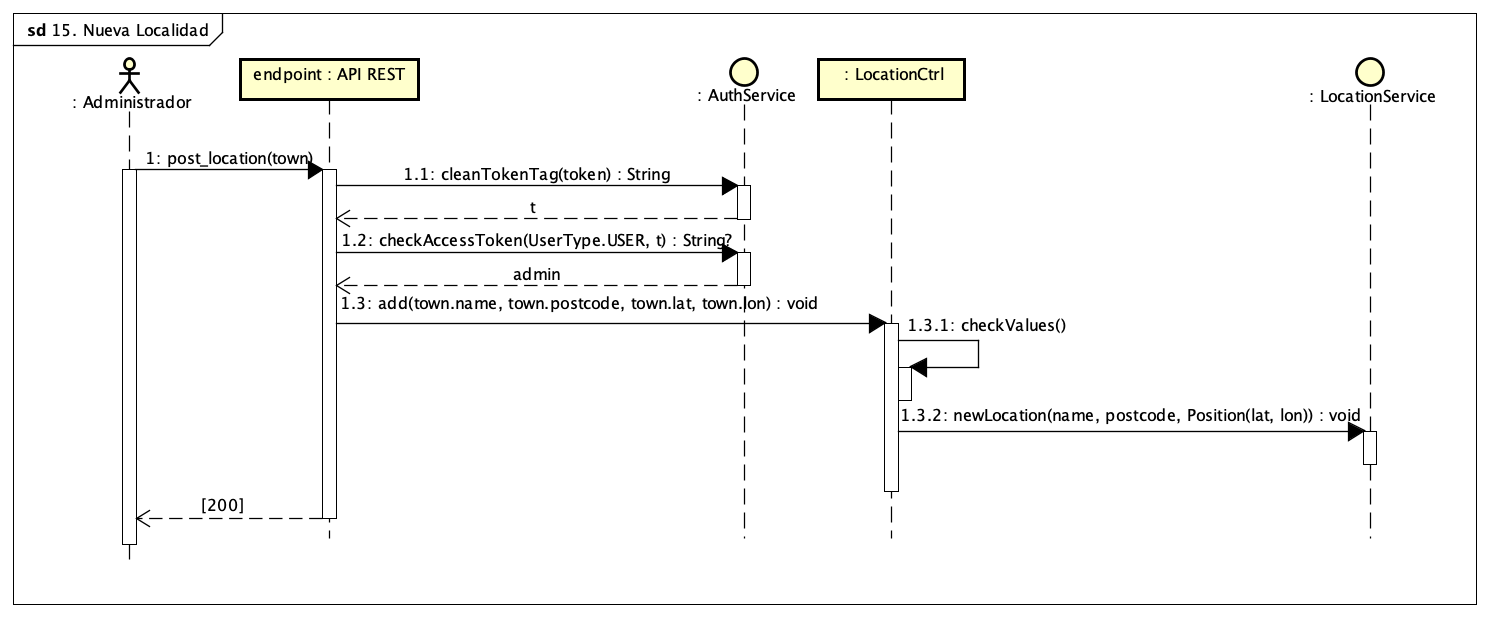
\includegraphics[width=14cm]{./img/sequence/diagram/NuevaLocalidad.png}
    \caption{Diagrama de secuencia DS15 - Adición de nueva localidad}
    \label{fig:seq.AddLocal}
\end{figure}

\subsubsection{Adición de un Nuevo Usuario}

Será necesario únicamente el nombre, documento nacional de identidad, y código postal.

\begin{figure}[H]
    \centering
    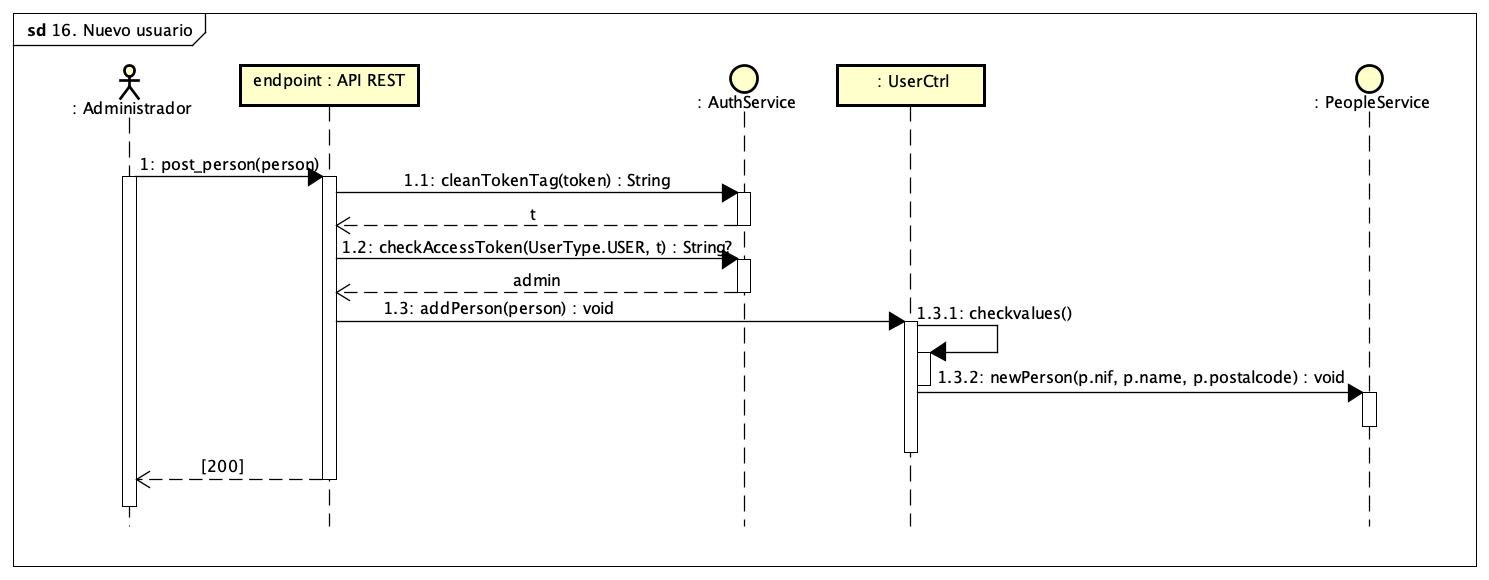
\includegraphics[width=14cm]{./img/sequence/diagram/NuevoUsuario.png}
    \caption{Diagrama de secuencia DS16 - Adición de nuevo usuario}
    \label{fig:seq.AddUser}
\end{figure}

\subsubsection{Asignación de Dispositivo}

Se creará únicamente una relación entre el usuario y el dispositivo, estando el dispositivo asociado a una determinada localidad a través del código postal de su poseedor.

\begin{figure}[H]
    \centering
    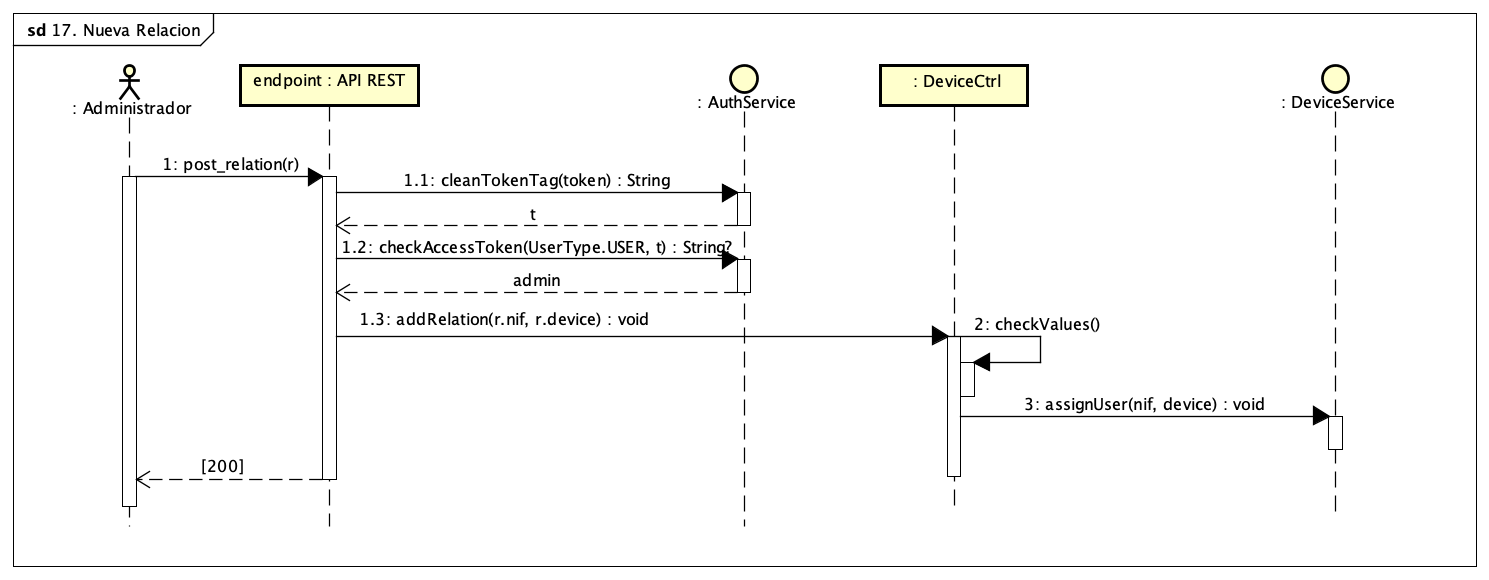
\includegraphics[width=14cm]{./img/sequence/diagram/NuevaRelacion.png}
    \caption{Diagrama de secuencia DS17 - Asignación de dispositivo}
    \label{fig:seq.AddUser}
\end{figure}

\subsubsection{Desasignación de Dispositivo}

Se debe permitir finalizar la relación entre un usuario y un dispositivo, de modo que el dispositivo pueda ser asociado a otro usuario en cuestión.

\begin{figure}[H]
    \centering
    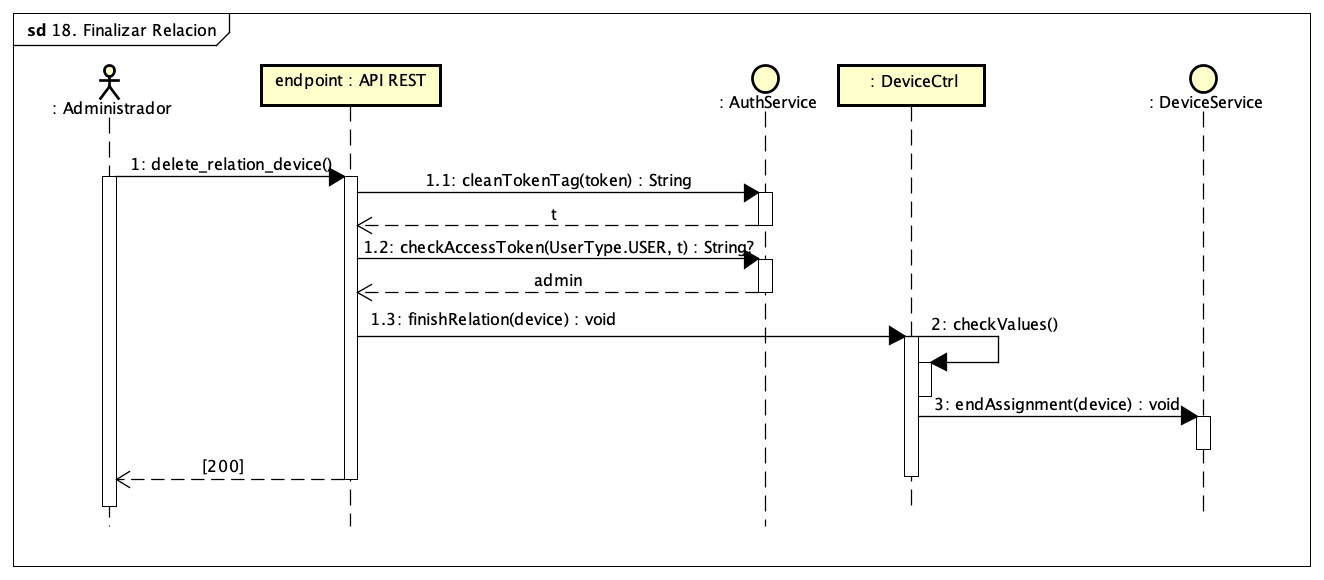
\includegraphics[width=14cm]{./img/sequence/diagram/FinalizarRelacion.png}
    \caption{Diagrama de secuencia DS18 - Desasignación de dispositivo}
    \label{fig:seq.AddUser}
\end{figure}

\subsubsection{Obtención de una Relación de Usuario}

Por motivos de necesidad, el administrador puede requerir conocer cual es la relación de un dispositivo específico. Por ello, a continuación se muestra cómo el sistema consigue la información.


\begin{figure}[H]
    \centering
    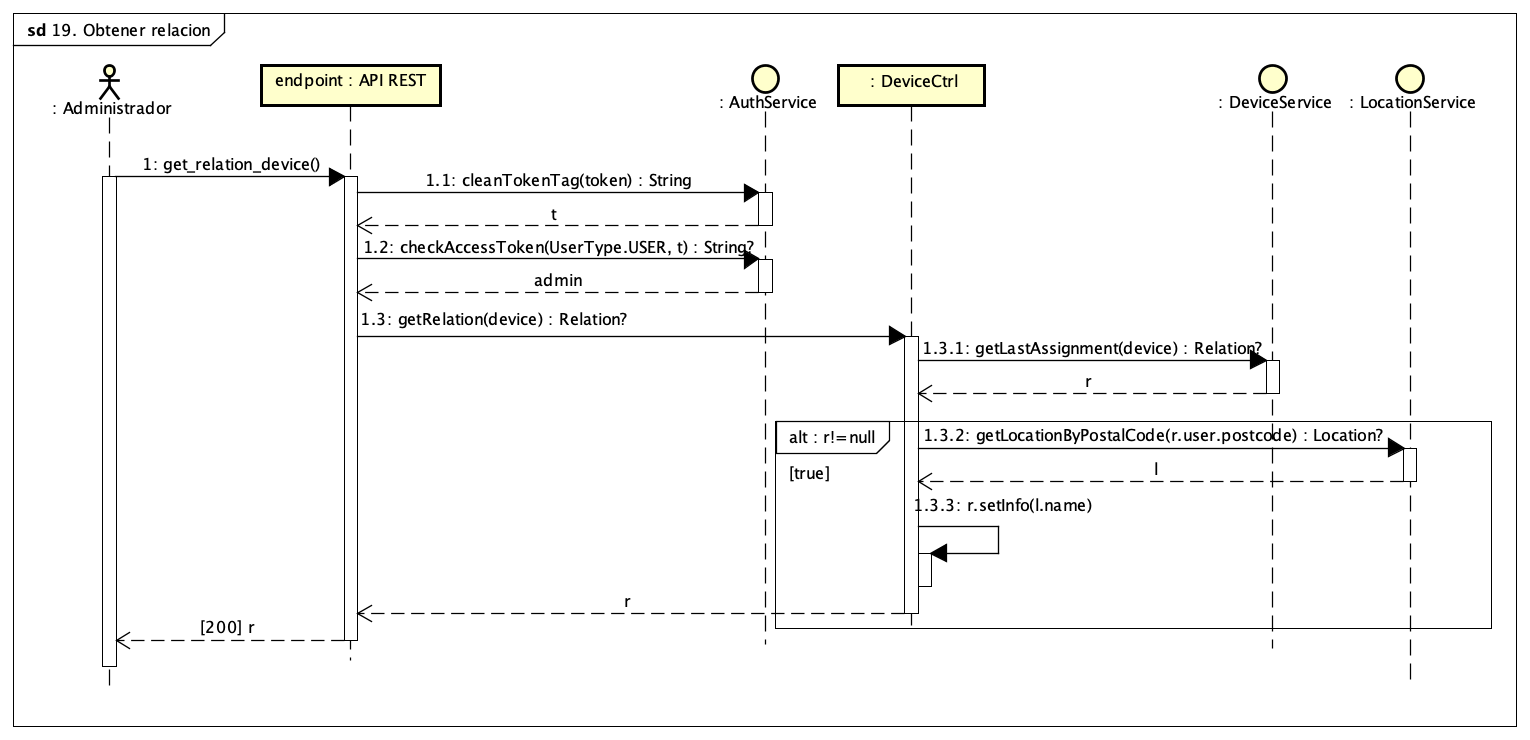
\includegraphics[width=14cm]{./img/sequence/diagram/ObtenerRelacion.png}
    \caption{Diagrama de secuencia DS19 - Obtención de relación}
    \label{fig:seq.AddUser}
\end{figure}
